\documentclass[intlimits]{beamer}

\mode<presentation>
{
  \usetheme{Madrid,Goettingen}
%  \usecolortheme{seahorse}
%  \usecolortheme{rose}
  \usecolortheme{rose,dolphin}
  \setbeamercovered{transparent}
  \setbeamertemplate{itemize item}[triangle]

  \setbeamertemplate{bibliography item}[book]

  \setbeamertemplate{navigation symbols}{}
  \setbeamertemplate{footline}
  {
    \leavevmode%
    \hbox{%
      \begin{beamercolorbox}[wd=.666666\paperwidth,ht=2.25ex,dp=1ex,center]{title in head/foot}%
        \usebeamerfont{title in head/foot}\insertshorttitle
      \end{beamercolorbox}%
      \begin{beamercolorbox}[wd=.333333\paperwidth,ht=2.25ex,dp=1ex,right] 
        {date in head/foot}%
        \usebeamerfont{date in head/foot}\insertshortdate{}\hspace*{2em}
        \insertframenumber{} / \inserttotalframenumber\hspace*{2ex}
    \end{beamercolorbox}}%
    \vskip0pt%
  }
}


% utf8 font & italian support
\usepackage[italian]{babel}
\usepackage{ucs}
\usepackage[utf8x]{inputenc}
\usepackage{lmodern}
\usepackage[T1]{fontenc}
\usepackage{textcomp}
\usepackage{mathrsfs}
\usepackage{graphicx}
\usepackage{subfigure}
\usepackage{comment}



\numberwithin{equation}{section}
\theoremstyle{plain}
  \newtheorem{teor}{Teorema}[section]
  \newtheorem{prop}[teor]{Proposizione}
  \newtheorem{cor}[teor]{Corollario}
  \newtheorem{cond}{Condizioni}[section]
\theoremstyle{definition}
  \newtheorem{defin}[teor]{Definizione}
\theoremstyle{remark}
  \newtheorem{esempio}[teor]{Esempio}
  \newtheorem{soluzione}[teor]{Soluzione}
  \newtheorem{esercizio}[teor]{Esercizio}
  \newtheorem{oss}[teor]{Osservazione}
  \newtheorem{prob}[teor]{Problema}
  \newtheorem{eqlog}[teor]{Equazione logistica}


\title[Metodi numerici per DDE]
{Metodi numerici per equazioni differenziali con ritardo}
\subtitle{Tesi di Laurea Triennale}

\author{Giampaolo Mele}
\institute{Università di Pisa}
\date{30 settembre 2011}



\begin{document}

\begin{frame}
\titlepage
\end{frame}


\begin{comment}
\section{Scaletta}


\begin{frame}{Scaletta}

\pause
\begin{itemize}[<+->]
 \item Presentazione del problema    
    \begin{itemize}
      \item Definizioni
      \item Equazione logistica
    \end{itemize}

 \item Risoluzione delle DDE
      \begin{itemize}
	\item Metodo di Bellman
	\item Metodo dei passi
      \end{itemize}


  \item Risoluzione numerica delle DDE
	\begin{itemize}
	 \item Estensioni continue dei metodi numerici per IVP
	 \item Regolarità della soluzione
	 \item Criteri di scelta della suddivisione
	 \item Approccio standard
	 \item Implementazione in matlab
	\end{itemize}
 

\end{itemize}

\end{frame}
\end{comment}



\section{Presentazione del problema}

\subsection{Definizioni}

\begin{frame}{DDE (delay differential equation)}
 Un'equazione differenziale con ritardo (DDE) è un problema della forma

\pause

\vspace{1cm}

\begin{defin}[DDE]
$$
\begin{cases}
 y'(t)=f(t,y(t),y \left( t-\tau \right))	\hspace{1cm}	t_0 \le t \le t_f		\\
 y(t)=\phi(t)					\hspace{4.35cm}		t \le t_0
\end{cases}
$$
\end{defin}

\pause

\vspace{1cm}

\begin{itemize}[<+->]
 \item $\tau=\tau(t,y(t))$ è detto ritardo
 \item $\phi(t)$ è detta storia
\end{itemize}

\end{frame}


\begin{frame}{Esistenza della soluzione}

\pause
\begin{cond}
 \begin{itemize}[<+->]
 \item $f(t,u,v)$ continua e lipschitziana sugli ultimi due argomenti
 \item $\tau(t,u)$  non negativa, continua e lipschitziana sul secondo argomento
 \item $\phi(t)$  continua e lipschitziana
\end{itemize}
\end{cond}

\pause

\vspace{1cm}
Sotto queste condizioni la soluzione della DDE esiste ed è unica
 
\end{frame}

\subsection{Equazione logistica}

\begin{frame}{Un esempio in biologia}
\pause

\begin{eqlog}

$$
\frac{d N}{d t} = r N(t) \left(1 - \frac{N(t)}{K} \right)
$$

\pause
L'equazione logistica [Verhulst 1838] descrive la crescita delle popolazioni 

\pause
\begin{itemize}[<+->]
 \item $N$ è il numero di individui della specie
 \item $r$ è il tasso di crescita
 \item $K$ è la capacità di carico della popolazione (numero massimo di individui 
	      che possono trovarsi in un determinato ambiente)
\end{itemize}

\end{eqlog}

\end{frame}


\begin{frame}{Incoerenze}

\pause
\begin{eqlog}
La soluzione di tale equazione è
$$
N(t)= \frac{K N_0 e^{rt}}{K+N_0(e^{rt}-1)}
$$
\pause
Questa è una funzione crescente, daltronde in natura a volte il numero di individui di una certa specie diminuisce oppure 
segue un andamento oscillatorio

\end{eqlog}

\end{frame}

\begin{frame}{Correzione con il fattore ritardo}

\pause

\begin{eqlog}[Hutchinson 1948]

$$
\frac{d N}{d t} = r N(t) \left(1 - \frac{N(t-\tau)}{K} \right)
$$

\end{eqlog}

\pause

\vspace{1cm}

\begin{prob}
 Come cambia la soluzione?
\end{prob}

\pause

\begin{esempio}
Fissiamo

\begin{itemize}
 \item $K=100$
 \item $r=0.1$
 \item $\phi(t)=3$
\end{itemize}

\end{esempio}

\end{frame}


\begin{frame}
 \begin{figure}[!ht]
\centering
\caption{Grafici al variare di $\tau$}
\subfigure[$\tau=5$ ]{
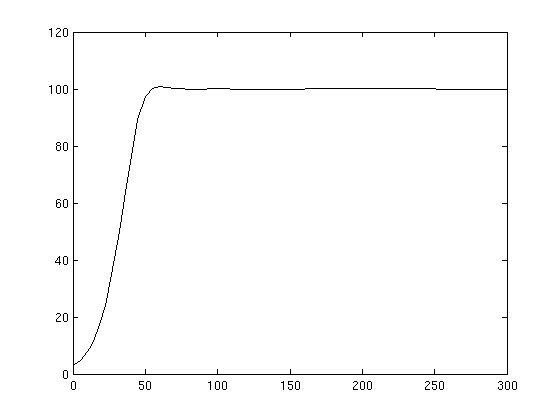
\includegraphics[width=4cm]{immagini/immagine2.png}}
\hspace{1mm}
\subfigure[$\tau=10$]{
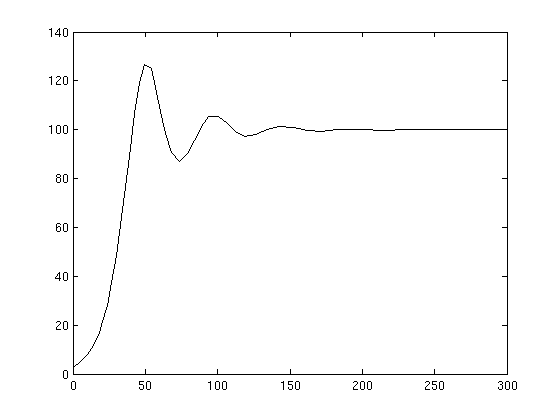
\includegraphics[width=4cm]{immagini/immagine3.png}}
\hspace{1mm}
\subfigure[$\tau=20$]{
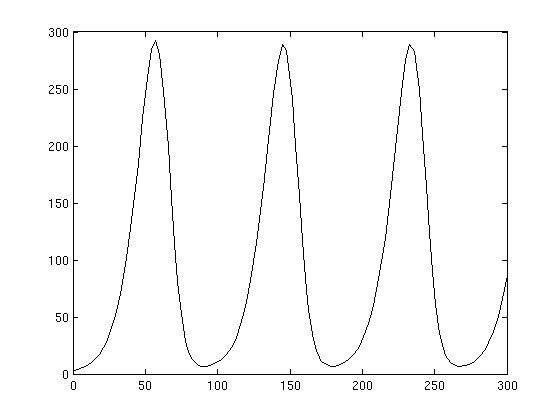
\includegraphics[width=4cm]{immagini/immagine4.png}}
\hspace{1mm}
\subfigure[$\tau=27$]{
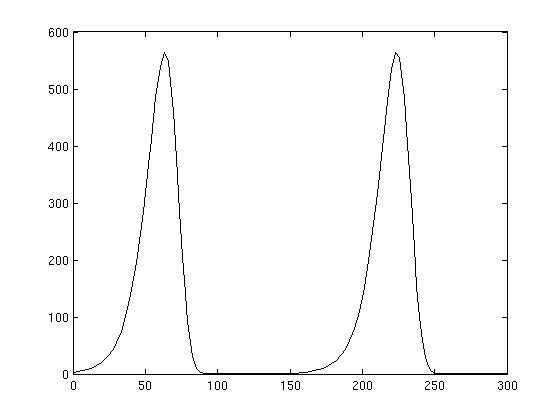
\includegraphics[width=4cm]{immagini/immagine5.png}}
\end{figure}
\end{frame}

\section{Metodo dei passi}

\subsection{Esempio}

\begin{frame}{Metodo dei passi}
\pause
\begin{esempio}
$$
\begin{cases}
 y'(t)=-y(t-1)	\hspace{1cm}		0 \le 	t \le N			\\
 y(t)=1		\hspace{3.3cm}			t \le 0
\end{cases}
$$
\end{esempio}
\pause
 
\vspace{1cm}

L'idea è di ricondurre la DDE a tanti problemi ai valori iniziali (IVP, initial value problem)

\end{frame}

\begin{frame}{Svolgimento}
\begin{esempio}
$$
\begin{cases}
 y'(t)=-y(t-1)	\hspace{1cm}		0 \le 	t \le N			\\
 y(t)=1		\hspace{3.3cm}			t \le 0
\end{cases}
$$
\end{esempio}
\pause
Per conoscere la soluzione in $[0,1]$ è sufficiente risolvere
\pause
\begin{block}{}
$$
\begin{cases}
 y_1'(t)=-1		 	\hspace{1cm}		t \in [0,1]	\\
 y_1(0)=1 
\end{cases}
$$
\end{block}


\pause
Ovvero

\begin{center}
 $y_1(t) = 1-t$
\end{center}

\pause
Per conoscerla in $[1 , 2]$ invece
\pause
\begin{block}{}
$$
\begin{cases}
 y_2'(t)=-y_1(t-1)= t-2		 	\hspace{1cm}		t \in [1,2]	\\
 y_2(1)=y_1(1)=0 
\end{cases}
$$
\end{block}



\end{frame}

\begin{frame}{Svolgimento}
\begin{esempio}
$$
\begin{cases}
 y'(t)=-y(t-1)	\hspace{1cm}		0 \le 	t \le N			\\
 y(t)=1		\hspace{3.3cm}			t \le 0
\end{cases}
$$
\end{esempio}

\pause
In generale possiamo determinare la soluzione per ricorrenza


\begin{block}{}
$$
\begin{cases}
y_0(t)		=	\phi(t)			\hspace{3cm}	t \le 0			\\
y_{i+1}'(t)	=	-y_i(t-1)		\hspace{1cm}	i \le t \le i+1		\\
y_{i+1}(i)	=	y_i(i)
\end{cases}
$$
\end{block}

\pause

La soluzione sarà l'incollamento delle $y_i$ ovvero
\pause
\begin{block}{}
$$
y(t)=y_i(t)	\hspace{1cm}	\mbox{se}	\hspace{1cm}	i \le t \le i+1
$$
\end{block}


\end{frame}

\begin{frame}{Svolgimento}
 \begin{esempio}
$$
\begin{cases}
 y'(t)=-y(t-1)	\hspace{1cm}		0 \le 	t \le N			\\
 y(t)=1		\hspace{3.3cm}			t \le 0
\end{cases}
$$
\end{esempio}

\begin{soluzione}
 $$
y(t)=
\begin{array}{lc lc}
\begin{cases}
\displaystyle
1-t												&	\hspace{0.7cm}	0 \le t \le 1	\\
\displaystyle
\frac{t^2}{2}-2t+\frac{3}{2}									&	\hspace{0.7cm}	1 \le t \le 2	\\
\displaystyle
-\frac{t^3}{6}+\frac{3}{2}t^2-4t+\frac{17}{6}							&	\hspace{0.7cm}	2 \le t \le 3	\\
\dots
\end{cases}
\end{array}
$$
\end{soluzione}
\end{frame}

\begin{frame}{Grafico della soluzione}
 
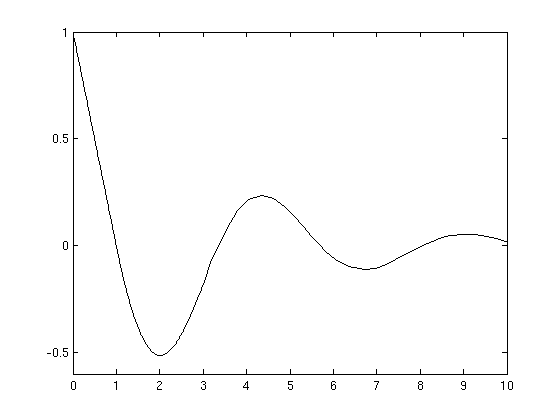
\includegraphics[width=10cm]{immagini/immagine6.png}


\end{frame}



\subsection{Caso generale}

\begin{frame}{Caso generale}
\pause
\begin{prob}
$$
\begin{cases}
 y'(t) = f(t,y(t),y(t- \tau (t,y(t)))	\hspace{1cm}	t_0 \le t \le t_f \\
 y(t)=\phi(t)				\hspace{5.5cm}	t \le t_0
\end{cases}
$$
\end{prob}
\pause
Data la suddivisione 
$$
\Delta= \left \{ t_0, t_1, \dots , t_n , \dots , t_N = t_f \right \}
$$
\pause
Risolvere la DDE equivale a risolvere un numero arbitrario di IVP
\end{frame}


\begin{frame}{Caso generale}
\pause
\begin{block}{DDE}
$$
\begin{cases}
 y'(t) = f(t,y(t),y(t- \tau (t,y(t)))	\hspace{1cm}	t_0 \le t \le t_f \\
 y(t)=\phi(t)				\hspace{5.5cm}	t \le t_0
\end{cases}
$$
\end{block}

\pause
\begin{block}{IVP associati alla DDE}
Data $\Delta$ per \hspace{0.3cm}	 $t_n \le t \le t_{n+1}$
$$
\begin{cases}
 y_{n+1}'(t)= f \left(t, y_{n+1}(t), x(t-\tau(t,y_{n+1}(t))) \right)	\\
 y_{n+1}(t_n)=y_n(t_n)
\end{cases}
$$
\end{block}
\pause
dove
\begin{block}{}
$$
\begin{array}{lc c}
  x(s):=
\begin{cases}
 \phi(s)	\hspace{1.75cm}	s \le t_0			\\
 y_{i}(s)	\hspace{0.5cm}	t_{i-1} \le s \le t_i 	
\end{cases}
&
y_0(t)=\phi(t)
\end{array}
$$
\end{block}

\end{frame}


\begin{frame}{Scelta di $\Delta$}

\pause
\begin{block}{}
 Quello che si vuole è che
$$
t-\tau < t_n		\hspace{2cm}	\forall t \in [t_n,t_{n+1}]
$$
\end{block}


\pause
\begin{block}{}
La condizione da imporre sulla suddivisione è
$$
t_{n+1} - t_n < \min{\tau}
$$
\end{block}

\pause
\begin{block}{Domanda}
 Cosa succede se $\tau$ si annulla?
\end{block}
\vspace{1cm}
\pause
 In realtà l'algoritmo si generalizza anche in questo caso...


 
\end{frame}


\section{Approccio standard}

\subsection{Estensioni continue di metodi numerici per IVP}

\begin{frame}{Problemi numerici}

\pause
\begin{block}{Domanda}
 La teoria sugli IVP è sufficiente?
\end{block}
\pause
\begin{oss}
 Di ogni IVP associato alla DDE è necessario conoscere un'approssimazione continua della soluzione, pertanto i classici metodi per 
 IVP (come ad esempio Eulero o i metodi di Runge-Kutta) non sono sufficienti dato che approssimano solo in alcuni punti la soluzione.
\end{oss}
\pause
Pertanto ci sono due possibilità:
\begin{itemize}
 \item Interpolare la soluzione
 \item Estendere i metodi numerici discreti a metodi numerici continui
\end{itemize}
\end{frame}

\begin{frame}{Definizioni}

\pause
\begin{block}{IVP}
$$
 \begin{cases}
  y'(t)=f(t,y(t))	\hspace{1cm}	t_0 \le t \le t_f	\\
  y(t_0)=y_0
 \end{cases}
$$
\end{block}
\pause
 \begin{defin}[Metodi numerici per IVP]
 Data una suddivisione $\Delta= \left \{ t_0, t_1, \dots , t_n , \dots , t_N = t_f \right \}$ definiamo 
un metodo numerico a $k$ passi come una successione
$$
\begin{array}{c lc}
y_{n+1} = & \alpha_{n,1} y_n + \dots +\alpha_{n,k} y_{n-k+1} \\
	  & + h_{n+1} \phi (y_n, \dots , y_{n-k+1})
\end{array}
\hspace{1cm}
0 \le n \le N-1
$$
dove $h_{n+1}=t_{n+1}-t_n$ e si suppongono noti i primi $k$ termini $y_0, \dots , y_{k-1}$.
Inoltre chiediamo che la funzione $\phi$ sia lipschitziana.
\end{defin}

\pause
 Quello che vogliamo è che $y_n \simeq y(t_n)$


\end{frame}


\begin{frame}{Definizioni}
 \begin{defin}[Estensione continua]
 Definiamo estensione continua (o interpolatore) di un metodo numerico una funzione $\eta(t)$ 
polinomiale a tratti definita dalle restrizioni su ogni intervallo $[t_n,t_{n+1}]$ di una interpolazione 
basata sui valori calcolati in un intervallo più amplio possibile $[t_{n-i_n},t_{n+j_n+1}]$ con 
$i_n,j_n \geq 0$ della forma
$$
\begin{array}{c lc}
\eta(t_n+\theta h_{n+1}) = & \beta_{n,1} (\theta) y_{n+j_n} + \dots + \beta_{n,j_n + i_n + 1} (\theta) y_{n-i_n} \\
			 & + h_{n+1} \Psi (y_{n+j_n}, \dots , y_{n-i_n}, \theta)
\end{array}
$$
dove $0 \le \theta \le 1$ e chiediamo che $\eta(t)$ sia continua, quindi
$$
\eta(t_n)=y_n	\hspace{1cm}	\mbox{e}	\hspace{1cm} \eta(t_{n+1})=y_{n+1}
$$
Inoltre chiediamo che la funzione $\Psi$ sia lipschitziana.
\end{defin}
\end{frame}

\begin{frame}{Consistenza}
 \begin{defin}[Consistenza di un metodo numerico]
 Un metodo numerico è consistente di ordine $p$ se per ogni IVP e per ogni suddivisione $\Delta$, 
 $p \geq 1$ è il più grande intero tale che 
 $$
 \| y(t_{n+1}) - \tilde{y}_{n+1}  \| = O(h_{n+1}^{p+1})
\hspace{1cm}	
\mbox{per}
\hspace{1cm}
0 \le n \le N-1
 $$
dove
$$
\begin{array}{c lc}
\tilde{y}_{n+1} = 	&	\alpha_{n,1} y(t_n) + \dots +\alpha_{n,k} y (t_{n-k+1}) \\ 
			&	+h_{n+1} \phi (y(t_n), \dots , y(t_{n-k+1}))
\end{array}
$$
\end{defin}
\end{frame}


\begin{frame}{Consistenza}
\begin{defin}[Consistenza di un'estensione continua]
Un'estensione continua è consistente di ordine $q$ se per ogni IVP e per ogni suddivisione $\Delta$, 
$q \geq 1$ è il più grande intero tale che 
 $$
\max_{t_n \le t \le t_{n+1}}
 \| y(t) - \tilde{\eta}(t)  \| = O(h_{n+1}^{q+1})
\hspace{0.8cm}	
\mbox{per}
\hspace{0.8cm}
0 \le n \le N-1
 $$
 dove
% riscalare con 

%\scalebox{0.9}{

$$
\small{
\begin{array}{l lc}
\tilde{\eta}(t_n+\theta h_{n+1}) =	 & \beta_{n,1} (\theta) y(t_{n+j_n}) + \dots + 
					    \beta_{n,j_n + i_n + 1} (\theta) y(t_{n-i_n})\\
					  & + h_{n+1} \Psi (y(t_{n+j_n}), \dots , y(t_{n-i_n}), \theta)	
\end{array}
}
$$
%}
\end{defin}
\end{frame}



\begin{frame}{Convergenza}
 \begin{defin}[Convergenza]
 Un metodo numerico è convergente di ordine $p$ se per ogni IVP e per ogni suddivisione $\Delta$, 
 posto $\displaystyle h = \max_{1 \le n \le N} t_n$ vale
$$
\max_{1 \le n \le N} \| y(t_n) -  y_n \| = O(h^p)
$$
la sua estensione continua è convergente di ordine $q$ se 
$$
\max_{t_0 \le t \le t_f} \| y(t) - \eta (t) \| = O(h^q)
$$
\end{defin}
\end{frame}

\begin{frame}{Matrice associata ad un metodo numerico}
$$
C_n=
\begin{pmatrix}
 \alpha_{n,1}	&	\alpha_{n,2}	&	\dots	&	\alpha_{n,k-1}	&	\alpha_{n,k}	\\
      1		&		0	&	\dots	&		0	&		0	\\
      0		&		1	&	\dots	&		0	&		0	\\
      \vdots	&	\vdots		&	\ddots	&	\vdots		&	\vdots		\\
      0		&		0	&	\dots	&		1	&		0
\end{pmatrix}
$$

\end{frame}


\begin{frame}{$0$-Stabilità}
 \begin{teor}
Sia 
$$
\begin{array}{c lc}
y_{n+1} =	&	 \alpha_{n,1} y_n + \dots +\alpha_{n,k} y_{n-k+1} \\
		&	+ h_{n+1} \phi (y_n, \dots , y_{n-k+1})
\end{array}
\hspace{1cm}
0 \le n \le N-1
$$
un metodo numerico a $k$ passi consistente di ordine $p$ e sia $C_n$
la sua matrice associata allora se
\begin{itemize}
 \item esiste una norma $\| \cdot \|_{*}$ tale che $\| C_n \|_{*} \le 1$
 \item la funzione $f$ (che definisce l'IVP) è di classe $C^p$
 \item i punti $y_0 \dots , y_{k-1}$ sono una approssimazione di ordine $p$ della soluzione esatta
\end{itemize}
allora il metodo è convergente di ordine $p$, inoltre se il metodo numerico ammette un'estensione 
continua consistente di ordine $q$ allora tale estensione è convergente di ordine 
$q'=\min \left \{ p , q+1 \right \} $
\end{teor}
\end{frame}

\begin{frame}{Esempio:Interpolazioni cubiche di Hermite}
 \begin{esempio}[Interpolazioni cubiche di Hermite]
Supponiamo di avere un metodo consistente di ordine $p \geq 3$, allora è possibile estendere questo 
metodo ad un metodo continuo consistente di ordine $3$ usando le interpolazioni 
cubiche di Hermite, ovvero calcolato 
$y_{n+1}$ approssimiamo 
la soluzione in $[t_{n},t_{n+1}]$ con 
$$
\begin{array}{c lc}
\eta(t_n+\theta h_{n+1}) = 	&	(1 - \theta) y_n + \theta y_{n+1}				\\
				&	+ \theta (\theta-1)[ (1- 2 \theta ) (y_{n+1} - y_n) 		\\
				&	+(\theta-1)h_n f (y_n,t_n) + \theta h_n f(y_{n+1},t_{n+1}) ] 
\end{array}
$$
\end{esempio}
\end{frame}


\begin{frame}{Metodi di Runge-Kutta}

\pause
I metodi di Runge-Kutta ad $\nu$ stadi sono definiti da

\pause
\begin{block}{Metodi di Runge-Kutta}
$$
\begin{cases}
\displaystyle
Y_{n+1}^i = y_n + h_{n+1} \sum_{j=1}^{\nu} a_{i,j} g(t_{n+1}^j,Y_{n+1}^j)
\hspace{1cm}
1 \le i \le \nu
\\
\displaystyle
y_{n+1} = y_n + h_{n+1} \sum_{i=1}^{\nu} b_i g (t_{n+1}^i,Y_{n+1}^i)
\end{cases}
$$
\end{block}


\end{frame}


\begin{frame}{Integratori di prima classe}

\pause
\begin{teor}
 Se un metodo di Runge-Kutta è consistente allora è convergente
\end{teor}

\pause
\begin{teor}[Esistenza degli interpolatori di prima classe]
Dato un metodo di Runge-Kutta con ordine di convergenza $p$ esiste un interpolatore con grado e ordine di convergenza 
$\lfloor \frac{p+1}{2} \rfloor$ 
\end{teor}
\end{frame}


\subsection{Localizzazione delle discontinuità}

\begin{frame}{Regolarità della soluzione}

\pause
\begin{block}{DDE}
$$
\begin{cases}
 y'(t)=f(t,y(t),y \left( t-\tau \right))	\hspace{1cm}	t_0 \le t \le t_f		\\
 y(t)=\phi(t)					\hspace{4.35cm}		t \le t_0
\end{cases}
$$
\end{block}

\pause
\begin{oss}
Se $f \in C^k$ allora la soluzione della DDE è una funzione $C^k$ a tratti
\end{oss}

\pause
Infatti può succedere l'incollamento tra la storia e la soluzione non sia $C^1$, ovvero

$$
y'(t_0)^- \ne y'(t_0)^+
$$
\pause
infatti
$$
\begin{array}{l}
y'(t_0)^- = \phi(t_0)											\\
y'(t_0)^+ = f(t_0, \phi(t_0),\phi(t_0 - \tau(t_0,\phi(t_0))))
\end{array}
$$
\end{frame}


\begin{frame}{Esempio}
\begin{block}{DDE}
$$
\begin{cases}
 y'(t)=-y(t-1)	\hspace{1cm}		0 \le 	t \le N			\\
 y(t)=1		\hspace{3.3cm}			t \le 0
\end{cases}
$$
\end{block}

\begin{soluzione}
 $$
y(t)=
\begin{array}{lc lc}
\begin{cases}
\displaystyle
1-t												&	\hspace{0.7cm}	0 \le t \le 1	\\
\displaystyle
\frac{t^2}{2}-2t+\frac{3}{2}									&	\hspace{0.7cm}	1 \le t \le 2	\\
\dots
\end{cases}
\end{array}
$$



\end{soluzione}

\pause

\begin{block}{}
 $$
\begin{array}{l}
y'(0)^-=\phi(0)=1 \\
y'(0)^+ = -y(0-1) =- 1
\end{array}
$$
\end{block}

\end{frame}



\begin{frame}{Grafico della soluzione}
 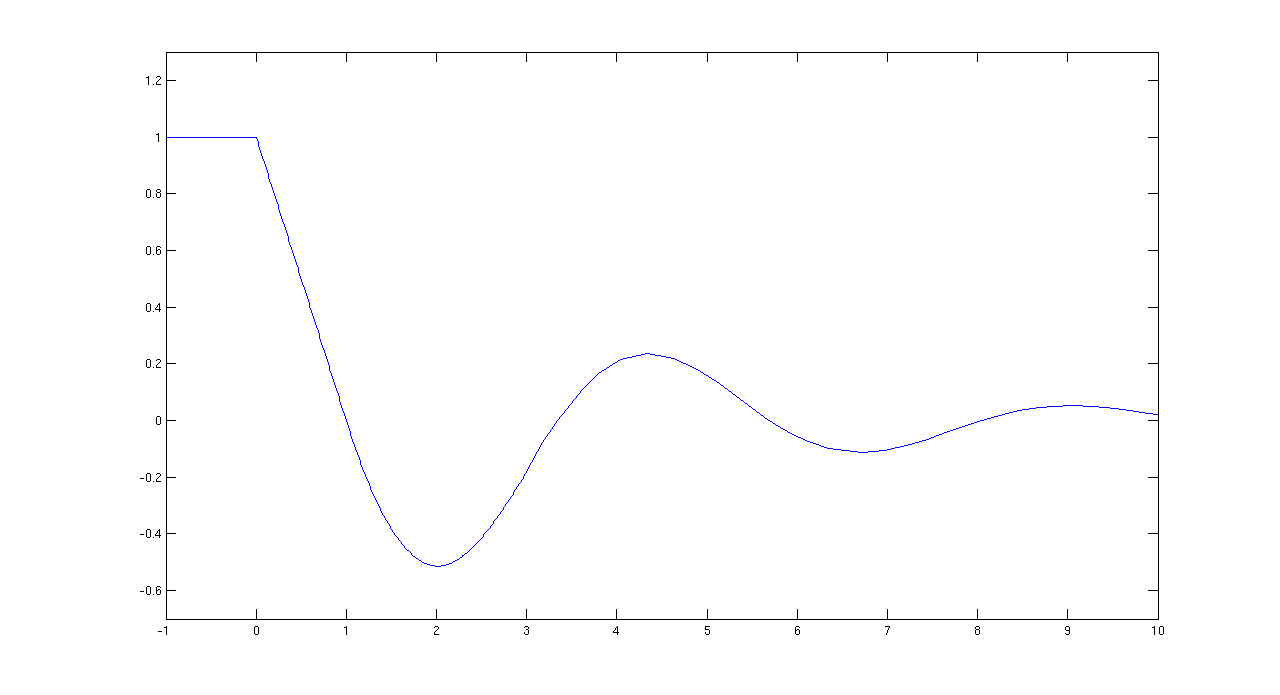
\includegraphics[width=10cm]{immagini/immagine12.png}
\end{frame}



\begin{frame}{Esempio}

\begin{block}{DDE}
$$
\begin{cases}
 y'(t)=-y(t-1)	\hspace{1cm}		0 \le 	t \le N			\\
 y(t)=1		\hspace{3.3cm}			t \le 0
\end{cases}
$$
\end{block}
\pause
\begin{block}{Propagazione delle discontinuità}
 Con gli stessi conti si trova che $y''$ è discontinua in $1$.
\\[0.5cm]
Non è difficile provare che $y^{(i+1)}$ è discontinua in $i$.
\end{block}

 
\end{frame}


\begin{frame}{Caso generale}
\pause
\begin{defin}[Discontinuità di ordine $k$]
Il punto $\xi$ è una discontinuità di ordine $k$ se per $0 \le s \le k-1$ si ha che $y^{(s)}(\xi)$ esiste e $y^{(k)}$ è lipschitziana 
e continua in un intorno di $\xi$, mentre $y^{(k+1)}$ è discontinua in $\xi$ 
\end{defin}

\pause

\begin{defin}[Argomento deviato]
$$
\alpha(t)=t-\tau(t,y(t))
$$ 
\end{defin}

\pause
\begin{block}{}
 Le (eventuali) discontinuità della soluzione sono dovute alla propagazione della (eventuale) discontinuità di ordine $0$ in $t_0$
\end{block}

\end{frame}

\begin{frame}{Caso generale}

\begin{prop}
Sia $\xi$ uno zero semplice di
$$
\alpha(\xi)=t_0
$$
Allora $y''$ è discontinua in $\xi$
\end{prop}

\pause

E' sufficiente derivare
\small{
$$
\begin{array}{l l}
y''(\xi)^+ = 	&	\frac{\partial f}{\partial t} \left( \xi,y(\xi),y(\alpha(\xi)) \right) + 					\\
		&	\frac{\partial f}{\partial y} \left( \xi,y(\xi),y(\alpha(\xi)) \right) y'(\xi)^+ +				\\
		&	\frac{\partial f}{\partial x} \left( \xi,y(\xi),y(\alpha(\xi)) \right) y'(\alpha(\xi))^+ \alpha'(\xi)		\\
\end{array}
$$

$$
\begin{array}{l l}
y''(\xi)^- = 	&	\frac{\partial f}{\partial t} \left( \xi,y(\xi),y(\alpha(\xi)) \right) + 					\\
		&	\frac{\partial f}{\partial y} \left( \xi,y(\xi),y(\alpha(\xi)) \right) y'(\xi)^- +				\\
		&	\frac{\partial f}{\partial x} \left( \xi,y(\xi),y(\alpha(\xi)) \right) y'(\alpha(\xi))^- \alpha'(\xi)		\\
\end{array}
$$
}


\end{frame}


\begin{frame}{Caso generale}

\begin{block}{}
Ripetendo gli stessi passaggi si trova che le $y'''$ è discontinua in $\xi'$ se questo è uno zero semplice di
$$
\alpha(\xi') = \xi
$$
\end{block}

\pause

Generalizzando

\begin{prop}[Discontinuità di grado $p$]
Le eventuali discontinuità di grado al più $p$ sono
$$
\begin{cases}
\alpha (\xi_{k,j}) = \xi_{k-1,i}\\
\xi_{0,1}=t_0
\end{cases}
\hspace{2cm}
1 \le i \le p	\hspace{0.5cm}
$$
\end{prop}

\end{frame}


\subsection{Convergenza del metodo dei passi}

\begin{frame}{Convergenza del metodo dei passi}

\begin{teor}

\begin{itemize}[<+->]
 \item Il metodo è $0$-stabile e consistente di ordine $p$
 \item L'interpolatore ha ordine di consistenza $q$
 \item La suddivisione $\Delta$ contiene tutte le discontinuità $\xi_i$ di ordine al più $p$
 \item L'interpolazione avviene in $[t_{n-i_n},t_{n+j_n+1}] \subseteq [\xi_i, \xi_{i+1}]$
\end{itemize}

\pause
Allora allora il metodo è convergente con ordine $q' = \min \left \{ p,q+1 \right \}$
$$
\max_{1 \le n \le N} \| y(t_n) - y_n \| = O(h^{q'})
$$
e anche l'interpolatore converge con lo stesso ordine
$$
\max_{t_0 \le t \le t_f} \| y(t) - \eta(t) \| = O(h^{q'})
$$

\end{teor}
 
\end{frame}


\section{Esperimenti numerici}

\begin{frame}{Domande}

\pause
\begin{block}{}
  Tutta questa teoria è necessaria?
\end{block}

\pause
\begin{block}{}
Cosa succede se $\Delta$ non contiene le discontinuità?
\end{block}

\end{frame}



\begin{frame}{Esperimenti numerici}
\pause
\begin{block}{DDE (Feldstein-Neves)}
$$
\displaystyle
\begin{cases}
\displaystyle
 y'(t)=\frac{1}{2 \sqrt{t}} y \left( y(t)-\sqrt{2} +1  \right)		 	\hspace{1cm} 		t \in [1,3]	\\
 y(t)=1										\hspace{5.2cm}		t \le 1
\end{cases}
$$
\end{block}
\pause
\begin{block}{Soluzione}
$$
y(t)=
\begin{cases}
\begin{array}{lc c}
\displaystyle
 \sqrt{t}										&	\hspace{1cm}		1 \le t \le 2	\\
\displaystyle
 \frac{t}{4}+\frac{1}{2}+\left( 1 - \frac{\sqrt{2}}{2} \right) \sqrt{t}			&	\hspace{1cm}		2 \le t \le 3
\end{array}
\end{cases}
$$
\end{block}

\end{frame}


\begin{frame}{Esperimenti numerici}
\pause
\begin{block}{}
Metodo di Runge-Kutta convergente di ordine 3 e mentre l'interpolatore è convergente di ordine 2.

\begin{center}
\renewcommand\arraystretch{1,5}
\begin{tabular}{c|cccc}
 $0$			&	$0$			&	$0$			&		$0$	\\
 $\frac{1}{3}$		&	$\frac{1}{3}$		&	$0$			&		$0$	\\
 $\frac{2}{3}$		&	$0$			&	$\frac{2}{3}$		&		$0$	\\
\hline
			&	$\frac{1}{4}$		&	$0$			&	$\frac{3}{4}$	\\
\end{tabular}
\renewcommand\arraystretch{1}
\hspace{2cm}
$
\renewcommand\arraystretch{1,5}
\begin{array}{lc}
 b_1(\theta) = -\frac{3}{4} \theta^2 + \theta									\\
 b_2(\theta) = 0												\\
 b_3(\theta) = \frac{3}{4} \theta^2
\end{array}
\renewcommand\arraystretch{1}
$
\end{center}
\end{block}



\end{frame}

\begin{frame}{Esperimenti numerici}

\begin{block}{}
\begin{itemize}[<+->]
 \item C'è una discontinuità in $2$
 \item Risolviamo il problema in $[1,3.11111]$
 \item $\Delta=\left \{1, 2, 3.11111 \right \}$
 \item $\Delta' = \left \{ 1, 1.7037, 2.4074, 3.1111 \right \}$
\end{itemize}
\end{block}

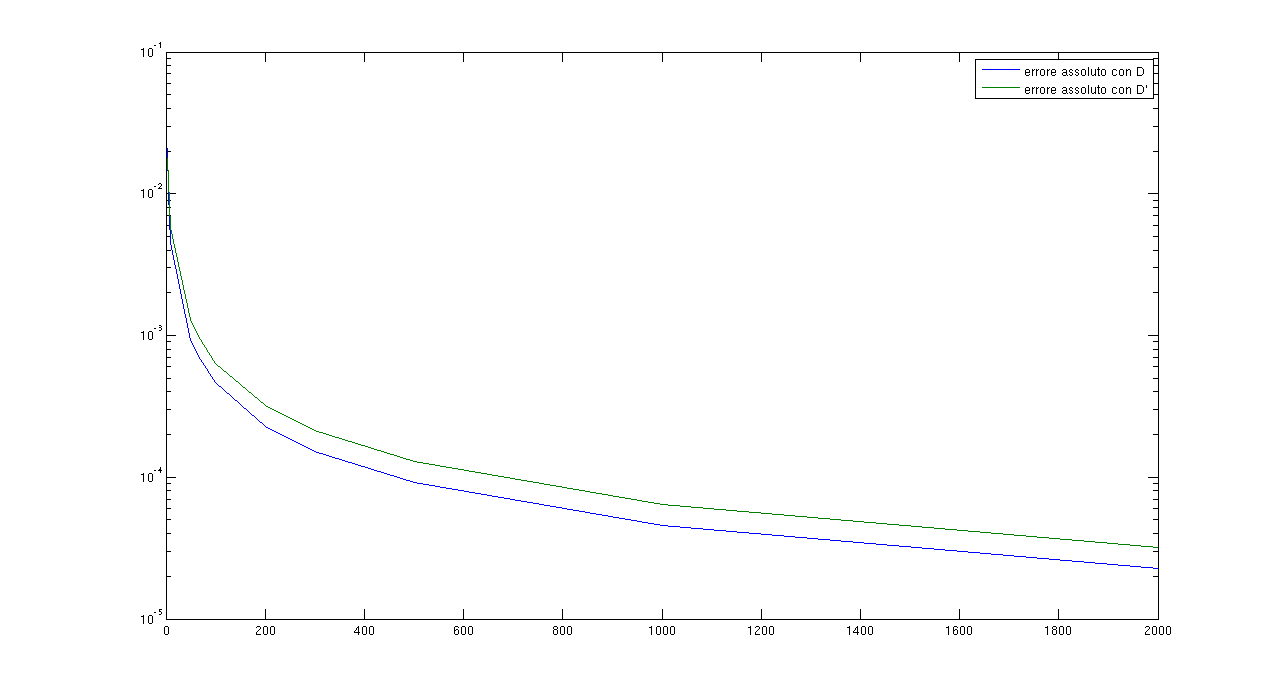
\includegraphics[width=10cm]{immagini/immagine11.png}


\end{frame}



\section{Conclusione}

\subsection{Differenze tra IVP e DDE}


\begin{frame}{Differenze tra IVP e DDE}

\pause
\begin{block}{Esempio}
 $$
  \begin{cases}
  y'(t)=-y(t-\tau)	\\
  y(t)=1		\hspace{3cm}	t \le 0
  \end{cases}
$$
\end{block}

\pause

\vspace{2cm}

\begin{block}{Cosa succede se:}
\begin{itemize}[<+->]
 \item $\tau=0$
 \item $\tau=1$
 \item $\tau=2$
\end{itemize}
\end{block}



\end{frame}


\begin{frame}{Differenze tra IVP e DDE}

\begin{figure}
\centering
\caption{Grafici al variare del ritardo}
\subfigure[$\tau=0,T=5$]{
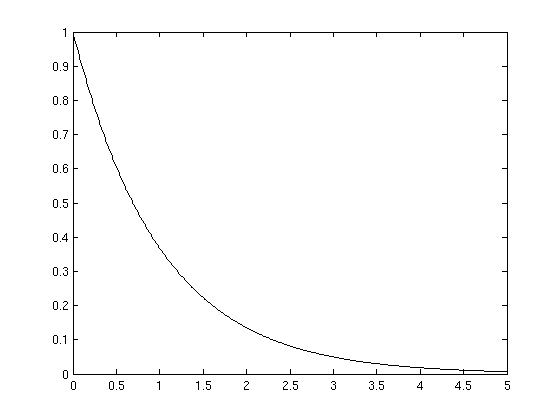
\includegraphics[width=3.75cm]{immagini/immagine7.png}}
\hspace{1mm}
\subfigure[$\tau=1,T=20$]{
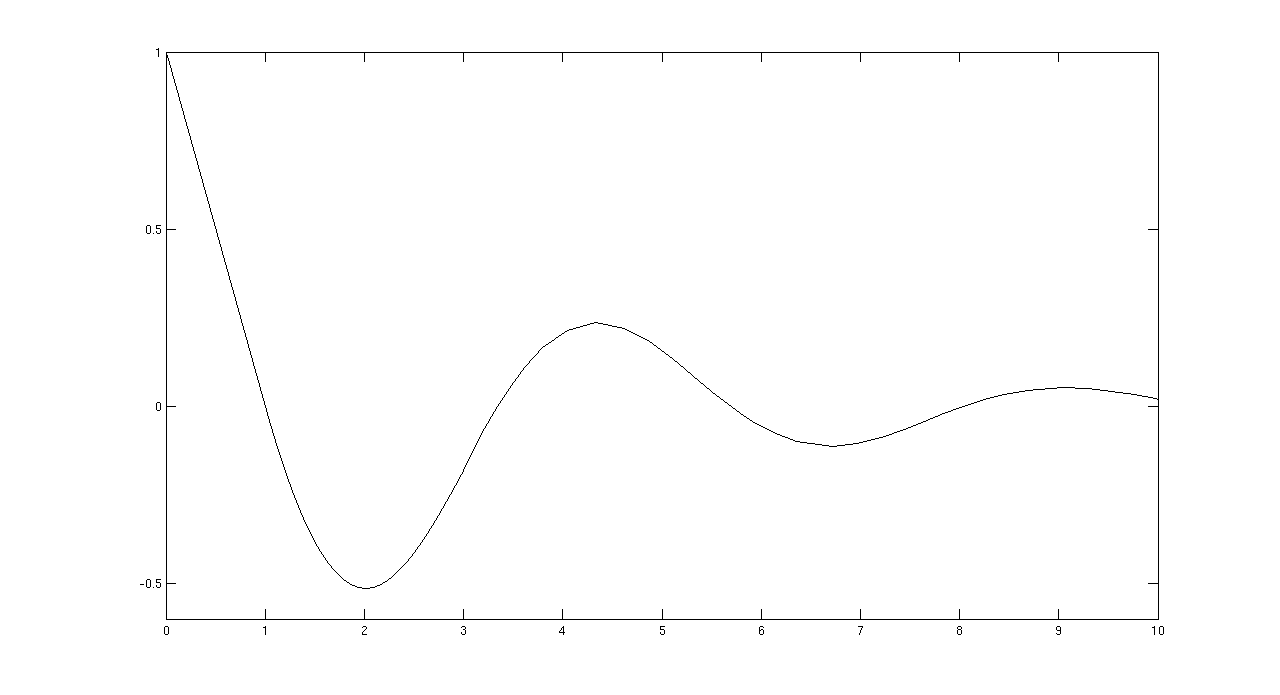
\includegraphics[width=5.25cm]{immagini/immagine8b.png}}
\hspace{1mm}
\subfigure[$\tau=2,T=50$]{
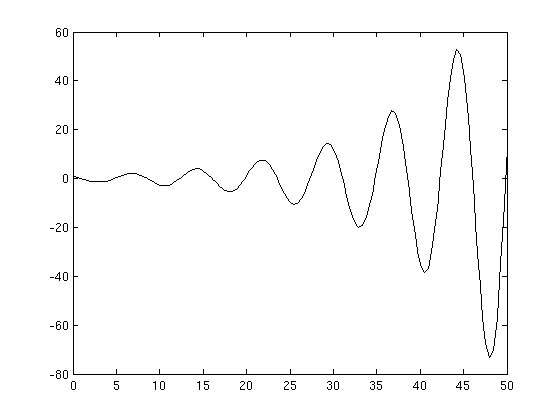
\includegraphics[width=3.75cm]{immagini/immagine9.png}}
\end{figure}

\end{frame}

\subsection{Conclusione}

\begin{frame}{Conclusione}

\pause
\begin{block}{}
 Il ritardo influisce sul comportamento qualitativo della soluzione
\end{block}

\pause
\begin{block}{}
 E' importante capire da cosa dipende il ritardo
\end{block}

\pause
\begin{block}{Equazione logistica}
 Il ritardo può dipendere da clima, temperatura, presenza di predatori,... \pause e può causare l'estinzione di una specie
\end{block}

\end{frame}


\begin{frame}{Fine}
 

    \begin{block}{}
    \begin{center}
     \Huge{
     Grazie per l'attenzione
      }
    \end{center}
    \end{block}

\end{frame}


\end{document}
